% Allow relative paths in included subfiles that are compiled separately
% See https://tex.stackexchange.com/questions/153312/
\providecommand{\main}{..}
\documentclass[\main/thesis.tex]{subfiles}

\begin{document}

\chapter{Autoencoder Embeddings with Improved Tree Ensemble}
\chaptermark{AENCXGB}
\label{chp:aencxgb}

In Chapter~\ref{chp:dl_autoenc} I discover that the autoencoder classification models provide worse overall challenge metrics compared to the gradient boosted tree model proposed in Chapter~\ref{chp:xgbensemble}, but are more sensitive in detecting \gls{irbbb}, \gls{lanfb}, and \gls{rad}.

This chapter explores the effectiveness of combining the autoencoder learned embeddings with the manually engineered features to train a new set of gradient boosted tree models.
I extend the approaches used in Chapters~\ref{chp:xgbensemble} and \ref{chp:dl_autoenc} with the following research questions:
\begin{enumerate}
    \item \label{question:xgb_aenc_avg_vs_lab} Rather than averaging the feature importances over all classifiers, will selecting top features with respect to the label-wise classifier improve the classification challenge metric?
    \item \label{question:xgb_aenc_embd_vs_no_embd} We have a deep learning approach for generating a fixed size embedding representation of a variable length \gls{ecg} record. Will incorporating the sequence embeddings from our deep learning autoencoder improve classification challenge metric?
    \item \label{question:xgb_aenc_embd_ratio} When adding the deep learning generated autoencoder embeddings, are they represented proportionally relative to the standard 12-lead derived heart beat, heart rate, and full waveform derived feature categories?
\end{enumerate}

\section{Methodology}

An initial processing step to convert the variable length features into fixed length input vectors is first applied on all \gls{ecg} records.
I combine the techniques applied in Section~\ref{ssec:xgb_feature_engineering} and Section~\ref{ssec:aenc_seq_embedding} to create ten different experiment configurations:
\begin{enumerate}
    \item \label{item:xgb_aenc_model_all_w_embd} \textbf{All Features with Embeddings}: I combine the feature engineering input vector (size 18,950) with the autoencoder sequence embedding vector (size 768) to create a combined input vector of size 19,718 and train an XGBClassifier for each of the 27 diagnosed labels.
    \item \label{item:xgb_aenc_model_all_no_embd} \textbf{All Features}: I use the feature engineering input vector of size 18,950 as the input to our label-wise XGBClassifier ensembles. This configuration is identical to the Phase 1 methodology described in Section~\ref{ssec:xgb_classification}.
    \item \label{item:xgb_aenc_model_avgd_top_1000_w_embd} \textbf{Averaged Top 1000 Features with Embeddings}: Using the trained models from Configuration~\ref{item:xgb_aenc_model_all_w_embd}, all label-wise classifier feature importances are averaged together before selecting the top 1,000 features.
    \item \label{item:xgb_aenc_model_top_1000_w_embd} \textbf{Top 1000 Features with Embeddings}: Starting from Configuration~\ref{item:xgb_aenc_model_all_w_embd}, I select the top 1,000 features for each diagnosis classifier and retrain a new set of 27 classifiers using the reduced feature set.
    \item \label{item:xgb_aenc_model_avgd_top_100_w_embd} \textbf{Averaged Top 100 Features with Embeddings}: Using the trained models from Configuration~\ref{item:xgb_aenc_model_all_w_embd}, all label-wise classifier feature importances are averaged together before selecting the top 100 features.
    \item \label{item:xgb_aenc_model_top_100_w_embd} \textbf{Top 100 Features with Embeddings}: Starting from Configuration~\ref{item:xgb_aenc_model_all_w_embd}, I select the 100 most important features for each diagnosis classifier and retrain a new set of 27 classifiers.
    \item \label{item:xgb_aenc_model_avgd_top_1000_no_embd} \textbf{Averaged Top 1000 Features}: Using Configuration~\ref{item:xgb_aenc_model_all_no_embd}, the classifier feature importances for all labels are averaged together to select the top 1,000 features. This configuration is identical to the Phase 2 methodology described in Section~\ref{ssec:xgb_classification}.
    \item \label{item:xgb_aenc_model_top_1000_no_embd} \textbf{Top 1000 Features}: Starting from Configuration~\ref{item:xgb_aenc_model_all_no_embd}, a new set of 27 classifiers is trained using the reduced top 1,000 most important features per label classifier.
    \item \label{item:xgb_aenc_model_avgd_top_100_no_embd} \textbf{Averaged Top 100 Features}: Using Configuration~\ref{item:xgb_aenc_model_all_no_embd}, the classifier feature importances for all labels are averaged together to select the top 100 features.
    \item \label{item:xgb_aenc_model_top_100_no_embd} \textbf{Top 100 Features}: Starting from Configuration~\ref{item:xgb_aenc_model_all_no_embd}, 27 classifiers are trained using the reduced top 100 most important features per label classifier.
\end{enumerate}

The significant differences distinguishing these approaches from the top 1000 features approach used in Section~\ref{ssec:xgb_classification} are that the importances of features for each of the labels are now evaluated independently, where the prior experiment used the same reduced set of features for all classifiers.
I further revise the inadequate dataset partitioning to use Monte Carlo cross-validation 20 times, randomly partitioning the available corpus of public data into 80\% training, 10\% validation, and 10\% test splits.

For each experiment configuration run, I train an \texttt{xgboost}~\cite{chen_xgboost_2016} binary classifier for each of the 27 diagnosed labels.
I use the dropout augmented regression tree booster proposed by Vinayak and Gilad-Bachrach~\cite{vinayak_dart_2015} and sample the training instances using probabilities proportional to the training gradients.
I use the scoring function reward matrix weights from Figure~\ref{fig:reward_matrix} as instance sample weights, capping positive examples to a threshold of 0.5.
I further scale the positive samples using the ratio of negative samples over positive samples for the given label and dataset split.
During training, if the evaluation set binary logistic regression loss fails to improve after 20 epochs of training, we early stop to mitigate overfitting on the training set.

\section{Results}

\begin{figure}[h]
    \centering
    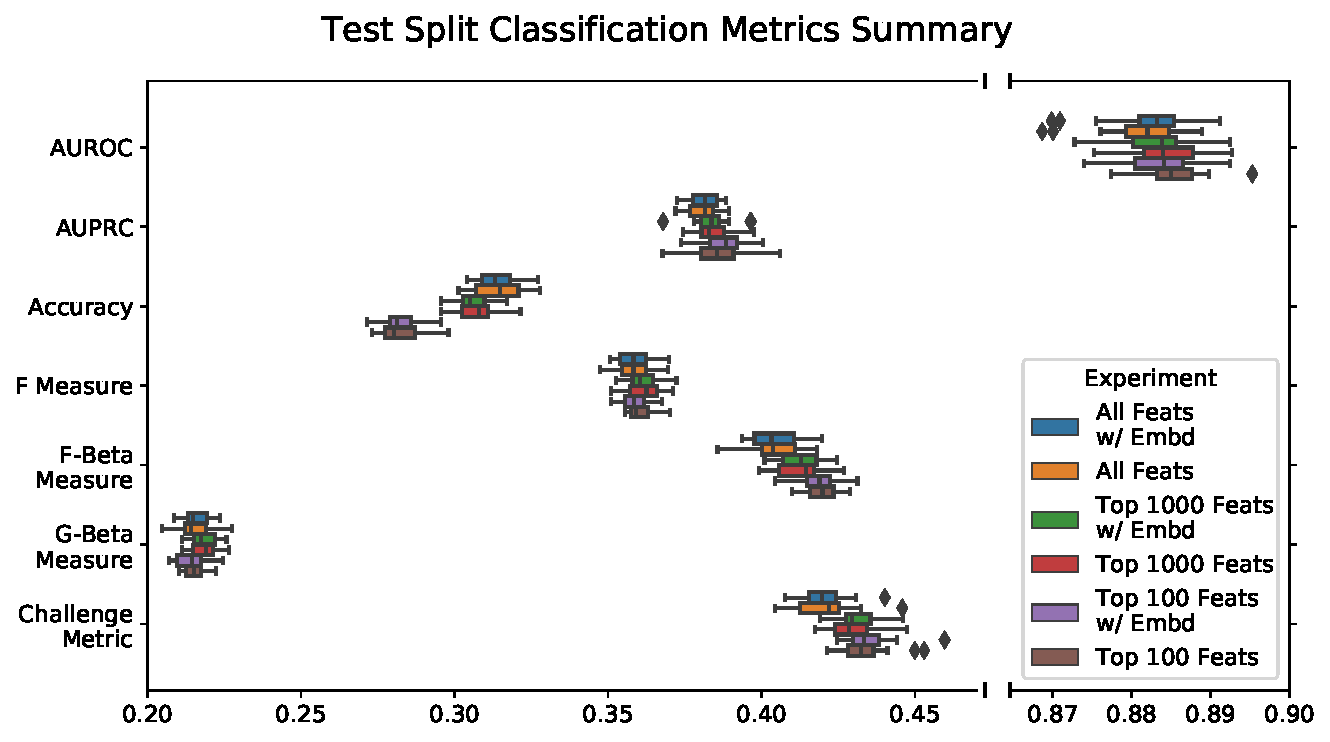
\includegraphics[trim={0.2cm 0.3cm 0.2cm 0.1cm},clip,width=\textwidth]{figure/xgb_aenc_classification_metrics.pdf}
    \caption[Test split classification metrics of XGB ensemble using all configurations of engineered features and autoencoder embeddings.]{Test split classification metrics of XGB ensemble using
    Configuration~\ref{item:xgb_aenc_model_all_w_embd}: All Features with Embeddings;
    Configuration~\ref{item:xgb_aenc_model_all_no_embd}: All Features;
    Configuration~\ref{item:xgb_aenc_model_avgd_top_1000_w_embd}: Averaged Top 1000 Features with Embeddings;
    Configuration~\ref{item:xgb_aenc_model_top_1000_w_embd}: Top 1000 Features with Embeddings;
    Configuration~\ref{item:xgb_aenc_model_avgd_top_100_w_embd}: Averaged Top 100 Features with Embeddings;
    Configuration~\ref{item:xgb_aenc_model_top_100_w_embd}: Top 100 Features with Embeddings;
    Configuration~\ref{item:xgb_aenc_model_avgd_top_1000_no_embd}: Averaged Top 1000 Features;
    Configuration~\ref{item:xgb_aenc_model_top_1000_no_embd}: Top 1000 Features;
    Configuration~\ref{item:xgb_aenc_model_avgd_top_100_no_embd}: Averaged Top 100 Features; and
    Configuration~\ref{item:xgb_aenc_model_top_100_no_embd}: Top 100 Features.
    }
    \label{fig:xgb_aenc_classification_metrics}
\end{figure}

\begin{table}[t]
    \caption{\label{tab:xgb_aenc_classification_metrics} Test split classification metrics mean ($\bar{x}$) and standard deviations ($\sigma$) for all experiment configurations. Bolded value indicates largest mean for metric category.}
    \vspace{2 mm}
    \centerline{\begin{tabular}{@{}c@{{ }}r@{{ }}c|c@{{ }}c@{{ }}c@{{ }}c@{{ }}c@{{ }}c@{{ }}c@{}}
    \multirow{2}{*}{\textbf{\#}}& \multirow{2}{*}{\textbf{Experiment}} & & \multirow{2}{*}{\textbf{AUROC}} & \multirow{2}{*}{\textbf{AUPRC}} & \multirow{2}{*}{\textbf{Accuracy}} & \multirow{2}{*}{\textbf{F Measure}} & \multirow{2}{*}{\textbf{F-Beta}} & \multirow{2}{*}{\textbf{G-Beta}} & \textbf{Challenge} \\
    & & & & & & & & & \textbf{Metric} \\ \hline
    % Configuration 1
    \multirow{2}{*}{\ref{item:xgb_aenc_model_all_w_embd}} & All Feats & $\bar{x}$ & $0.8821$ & $0.3813$ & $0.3137$ & $0.3587$ & $0.4047$ & $0.2160$ & $0.4207$ \\
    & w/ Embd & $\sigma$ & $5.3 \times 10^{-3}$ & $4.9 \times 10^{-3}$ & $6.8 \times 10^{-3}$ & $5.9 \times 10^{-3}$ & $8.1 \times 10^{-3}$ & $3.9 \times 10^{-3}$ & $7.7 \times 10^{-3}$
    \\ \hline
    % Configuration 2
    \multirow{2}{*}{\ref{item:xgb_aenc_model_all_no_embd}} & \multirow{2}{*}{All Feats} & $\bar{x}$ & $0.8815$ & $0.3809$ & \textbf{0.3139} & $0.3582$ & $0.4036$ & $0.2150$ & $0.4206$ \\
    & & $\sigma$ & $5.5 \times 10^{-3}$ & $5.0 \times 10^{-3}$ & $7.9 \times 10^{-3}$ & $6.0 \times 10^{-3}$ & $8.6 \times 10^{-3}$ & $5.2 \times 10^{-3}$ & $1.0 \times 10^{-2}$ \\ \hline
    % Configuration 3
    \multirow{2}{*}{\ref{item:xgb_aenc_model_avgd_top_1000_w_embd}} & Avg Top 1000 & $\bar{x}$ & \textbf{0.8876} & \textbf{0.3900} & $0.3068$ & $0.3637$ & $0.4165$ & \textbf{0.2194} & \textbf{0.4366} \\
    & Feats w/ Embd & $\sigma$ & $4.6 \times 10^{-3}$ & $5.5 \times 10^{-3}$ & $6.5 \times 10^{-3}$ & $4.5 \times 10^{-3}$ & $6.0 \times 10^{-3}$ & $4.3 \times 10^{-3}$ & $7.1 \times 10^{-3}$ \\ \hline
    % Configuration 4
    \multirow{2}{*}{\ref{item:xgb_aenc_model_top_1000_w_embd}} & Top 1000 Feats & $\bar{x}$ & $0.8836$ & $0.3837$ & $0.3062$ & $0.3613$ & $0.4128$ & $0.2183$ & $0.4316$ \\
    & w/ Embd & $\sigma$ & $4.8 \times 10^{-3}$ & $6.4 \times 10^{-3}$ & $5.4 \times 10^{-3}$ & $5.4 \times 10^{-3}$ & $6.7 \times 10^{-3}$ & $4.3 \times 10^{-3}$ & $7.0 \times 10^{-3}$ \\ \hline
    % Configuration 5
    \multirow{2}{*}{\ref{item:xgb_aenc_model_avgd_top_100_w_embd}} & Avg Top 100 & $\bar{x}$ & $0.8740$ & $0.3740$ & $0.2800$ & $0.3482$ & $0.4062$ & $0.2066$ & $0.4215$ \\
    & Feats w/ Embd & $\sigma$ & $5.1 \times 10^{-3}$ & $7.8 \times 10^{-3}$ & $9.7 \times 10^{-3}$ & $6.5 \times 10^{-3}$ & $6.8 \times 10^{-3}$ & $5.2 \times 10^{-3}$ & $9.9 \times 10^{-3}$ \\ \hline
    % Configuration 6
    \multirow{2}{*}{\ref{item:xgb_aenc_model_top_100_w_embd}} & Top 100 Feats & $\bar{x}$ & $0.8836$ & $0.3876$ & $0.2820$ & $0.3588$ & $0.4190$ & $0.2143$ & $0.4348$ \\
    & w/ Embd & $\sigma$ & $4.9 \times 10^{-3}$ & $7.0 \times 10^{-3}$ & $6.2 \times 10^{-3}$ & $5.1 \times 10^{-3}$ & $6.8 \times 10^{-3}$ & $4.9 \times 10^{-3}$ & $7.8 \times 10^{-3}$ \\ \hline
    % Configuration 7
    \multirow{2}{*}{\ref{item:xgb_aenc_model_avgd_top_1000_no_embd}} & Avg Top & $\bar{x}$ & $0.8871$ & $0.3890$ & $0.3085$ & \textbf{0.3640} & $0.4165$ & $0.2187$ & $0.4358$ \\
    & 1000 Feats & $\sigma$ & $5.1 \times 10^{-3}$ & $6.7 \times 10^{-3}$ & $6.6 \times 10^{-3}$ & $6.2 \times 10^{-3}$ & $8.1 \times 10^{-3}$ & $5.6 \times 10^{-3}$ & $8.1 \times 10^{-3}$ \\ \hline
    % Configuration 8
    \multirow{2}{*}{\ref{item:xgb_aenc_model_top_1000_no_embd}} & \multirow{2}{*}{Top 1000 Feats} & $\bar{x}$ & $0.8843$ & $0.3836$ & $0.3075$ & $0.3619$ & $0.4126$ & $0.2179$ & $0.4295$ \\
    & & $\sigma$ & $5.2 \times 10^{-3}$ & $5.6 \times 10^{-3}$ & $6.4 \times 10^{-3}$ & $5.2 \times 10^{-3}$ & $7.5 \times 10^{-3}$ & $4.4 \times 10^{-3}$ & $8.1 \times 10^{-3}$ \\ \hline
    % Configuration 9
    \multirow{2}{*}{\ref{item:xgb_aenc_model_avgd_top_100_no_embd}} & Avg Top & $\bar{x}$ & $0.8714$ & $0.3748$ & $0.2800$ & $0.3471$ & $0.4035$ & $0.2057$ & $0.4195$ \\
    & 100 Feats & $\sigma$ & $6.7 \times 10^{-3}$ & $6.4 \times 10^{-3}$ & $5.3 \times 10^{-3}$ & $4.6 \times 10^{-3}$ & $6.2 \times 10^{-3}$ & $5.1 \times 10^{-3}$ & $7.8 \times 10^{-3}$ \\ \hline
    % Configuration 10
    \multirow{2}{*}{\ref{item:xgb_aenc_model_top_100_no_embd}} & \multirow{2}{*}{Top 100 Feats} & $\bar{x}$ & $0.8848$ & $0.3857$ & $0.2830$ & $0.3604$ & \textbf{0.4198} & $0.2150$ & $0.4335$ \\
    & & $\sigma$ & $4.5 \times 10^{-3}$ & $8.5 \times 10^{-3}$ & $7.5 \times 10^{-3}$ & $4.0 \times 10^{-3}$ & $5.3 \times 10^{-3}$ & $3.3 \times 10^{-3}$ & $8.2 \times 10^{-3}$ \\
    \end{tabular}}
\end{table}

\begin{figure}[t]
    \centering
    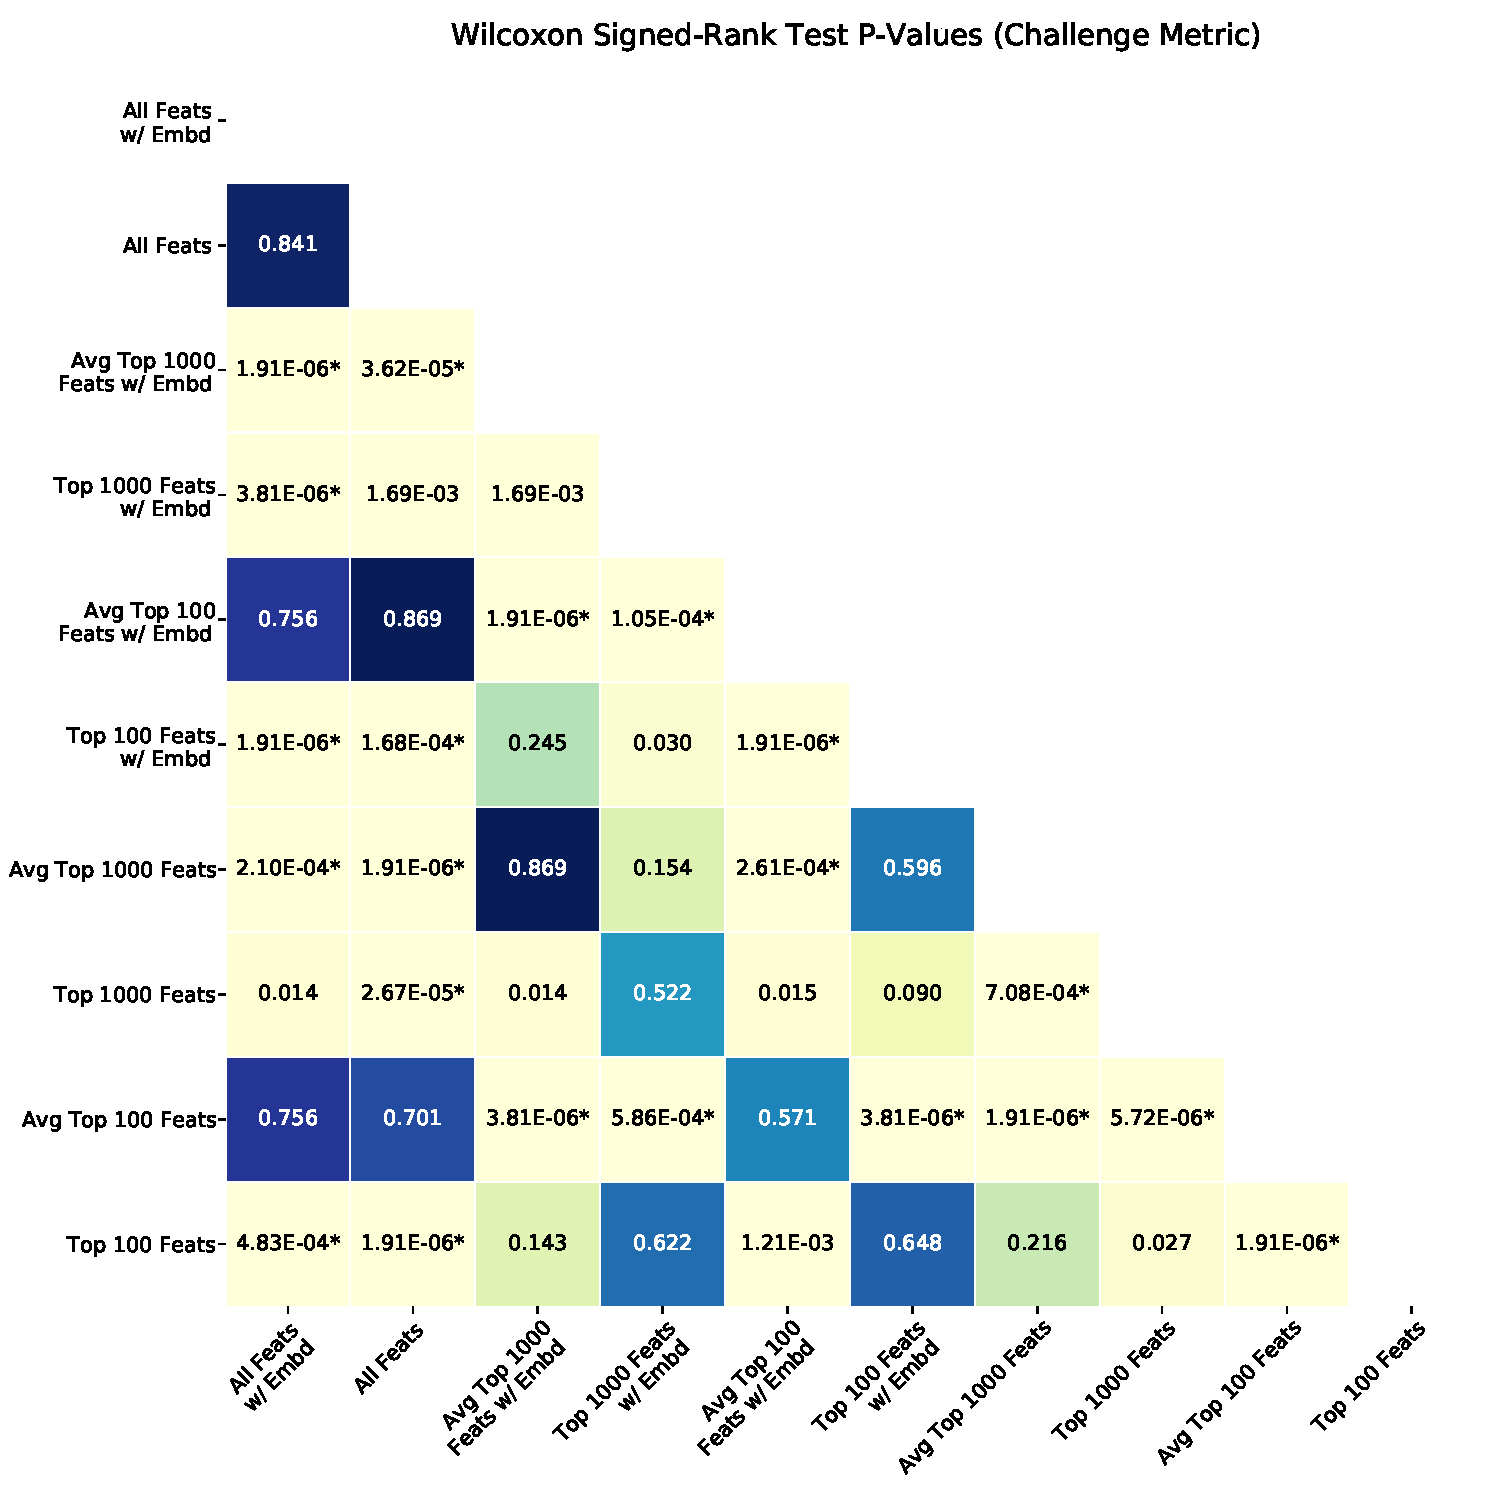
\includegraphics[width=12cm]{figure/xgb_aenc_wilcoxon_srt_p_vals.pdf}
    \caption[Wilcoxon signed-rank test P-values, comparing test split challenge metric distributions of all 6 experiment configurations.]{Wilcoxon signed-rank test P-values, comparing test split challenge metric distributions of all 6 experiment configurations. Asterisk indicates significantly different challenge metric distribution at a confidence level of 0.1\%.}
    \label{fig:xgb_aenc_wilcoxon_srt_p_vals}
\end{figure}

Refer to Figure~\ref{fig:xgb_aenc_classification_metrics} and Table~\ref{tab:xgb_aenc_classification_metrics} for the test set split classification metric summaries for all experiment configurations.
The experiment configuration with the largest mean challenge score is the ``Top 100 Features with Embeddings", or the top 100 features from both the engineered and autoencoder sources.
I apply the Wilcoxon signed-rank test to determine if the challenge metrics from Configuration~\ref{item:xgb_aenc_model_top_100_w_embd} are statistically different than all of the other experiment configurations.
See Figure~\ref{fig:xgb_aenc_wilcoxon_srt_p_vals} for the Wilcoxon signed-rank test evaluated on all configuration pairs.

\subsection{Averaged vs Labelwise Feature Selection}
To address Question~\ref{question:xgb_aenc_avg_vs_lab}, if selecting important features by classifier is an improvement to just averaging all of the classifiers together, we should see the averaged top feature configurations perform worse than the top feature configurations.
With a confidence of $0.1\%$, I analyze the relevant configuration pairs:
\begin{itemize}
    \item \textbf{1000 Features with Embeddings}: Configuration~\ref{item:xgb_aenc_model_avgd_top_1000_w_embd} has a higher challenge score than Configuration~\ref{item:xgb_aenc_model_top_1000_w_embd}, but it is not statistically significant.
    \item \textbf{100 Features with Embeddings}: Configuration~\ref{item:xgb_aenc_model_avgd_top_100_w_embd} has a lower challenge score than Configuration~\ref{item:xgb_aenc_model_top_100_w_embd}, and \emph{it is statistically significant}, suggesting labelwise selection of features increases the challenge metric.
    \item \textbf{1000 Features}: Configuration~\ref{item:xgb_aenc_model_avgd_top_1000_no_embd} has a higher challenge score than Configuration~\ref{item:xgb_aenc_model_top_1000_no_embd}, and \emph{it is statistically significant}, suggesting labelwise selection of features decreases the challenge metric.
    \item \textbf{100 Features}: Configuration~\ref{item:xgb_aenc_model_avgd_top_100_no_embd} has a lower challenge score than Configuration~\ref{item:xgb_aenc_model_top_100_no_embd}, and \emph{it is statistically significant}, suggesting labelwise selection of features increases the challenge metric.
\end{itemize}

The results suggest that labelwise selection of features improves the challenge metric when the feature pruning is aggressive (top 100), but does not have a significant effect when the feature pruning is not aggressive (top 1000).

\subsection{Adding Embeddings vs Without Embeddings}
To answer Question~\ref{question:xgb_aenc_embd_vs_no_embd}, if incorporating the autoencoder embeddings improves the classifier, we should see the configurations using embeddings outperform the configurations without embeddings in the challenge metric. 
I analyze the relevant configuration pairs, using a confidence of $0.1\%$:
\begin{itemize}
    \item \textbf{Averaged Top 1000 Features}: Configuration~\ref{item:xgb_aenc_model_avgd_top_1000_w_embd} has a higher challenge score than Configuration~\ref{item:xgb_aenc_model_avgd_top_1000_no_embd}, but it is not statistically significant.
    \item \textbf{Top 1000 Features}: Configuration~\ref{item:xgb_aenc_model_top_1000_w_embd} has a higher challenge score than Configuration~\ref{item:xgb_aenc_model_top_1000_no_embd}, but it is not statistically significant.
    \item \textbf{Averaged Top 100 Features}: Configuration~\ref{item:xgb_aenc_model_avgd_top_100_w_embd} has a higher challenge score than Configuration~\ref{item:xgb_aenc_model_avgd_top_100_no_embd}, but it is not statistically significant.
    \item \textbf{Top 100 Features}: Configuration~\ref{item:xgb_aenc_model_top_100_w_embd} has a higher challenge score than Configuration~\ref{item:xgb_aenc_model_top_100_no_embd}, but it is not statistically significant.
\end{itemize}

The results suggest that although adding autoencoder embeddings into the input vector as additional representation of the \gls{ecg} record improves the average classification metric of the experiments, the increased classification metric is not statistically significant.

\subsection{Embedding Feature Importances}
\label{ssec:xgb_aenc_embd_feat_importances}

\begin{figure}[t]
    \centering
    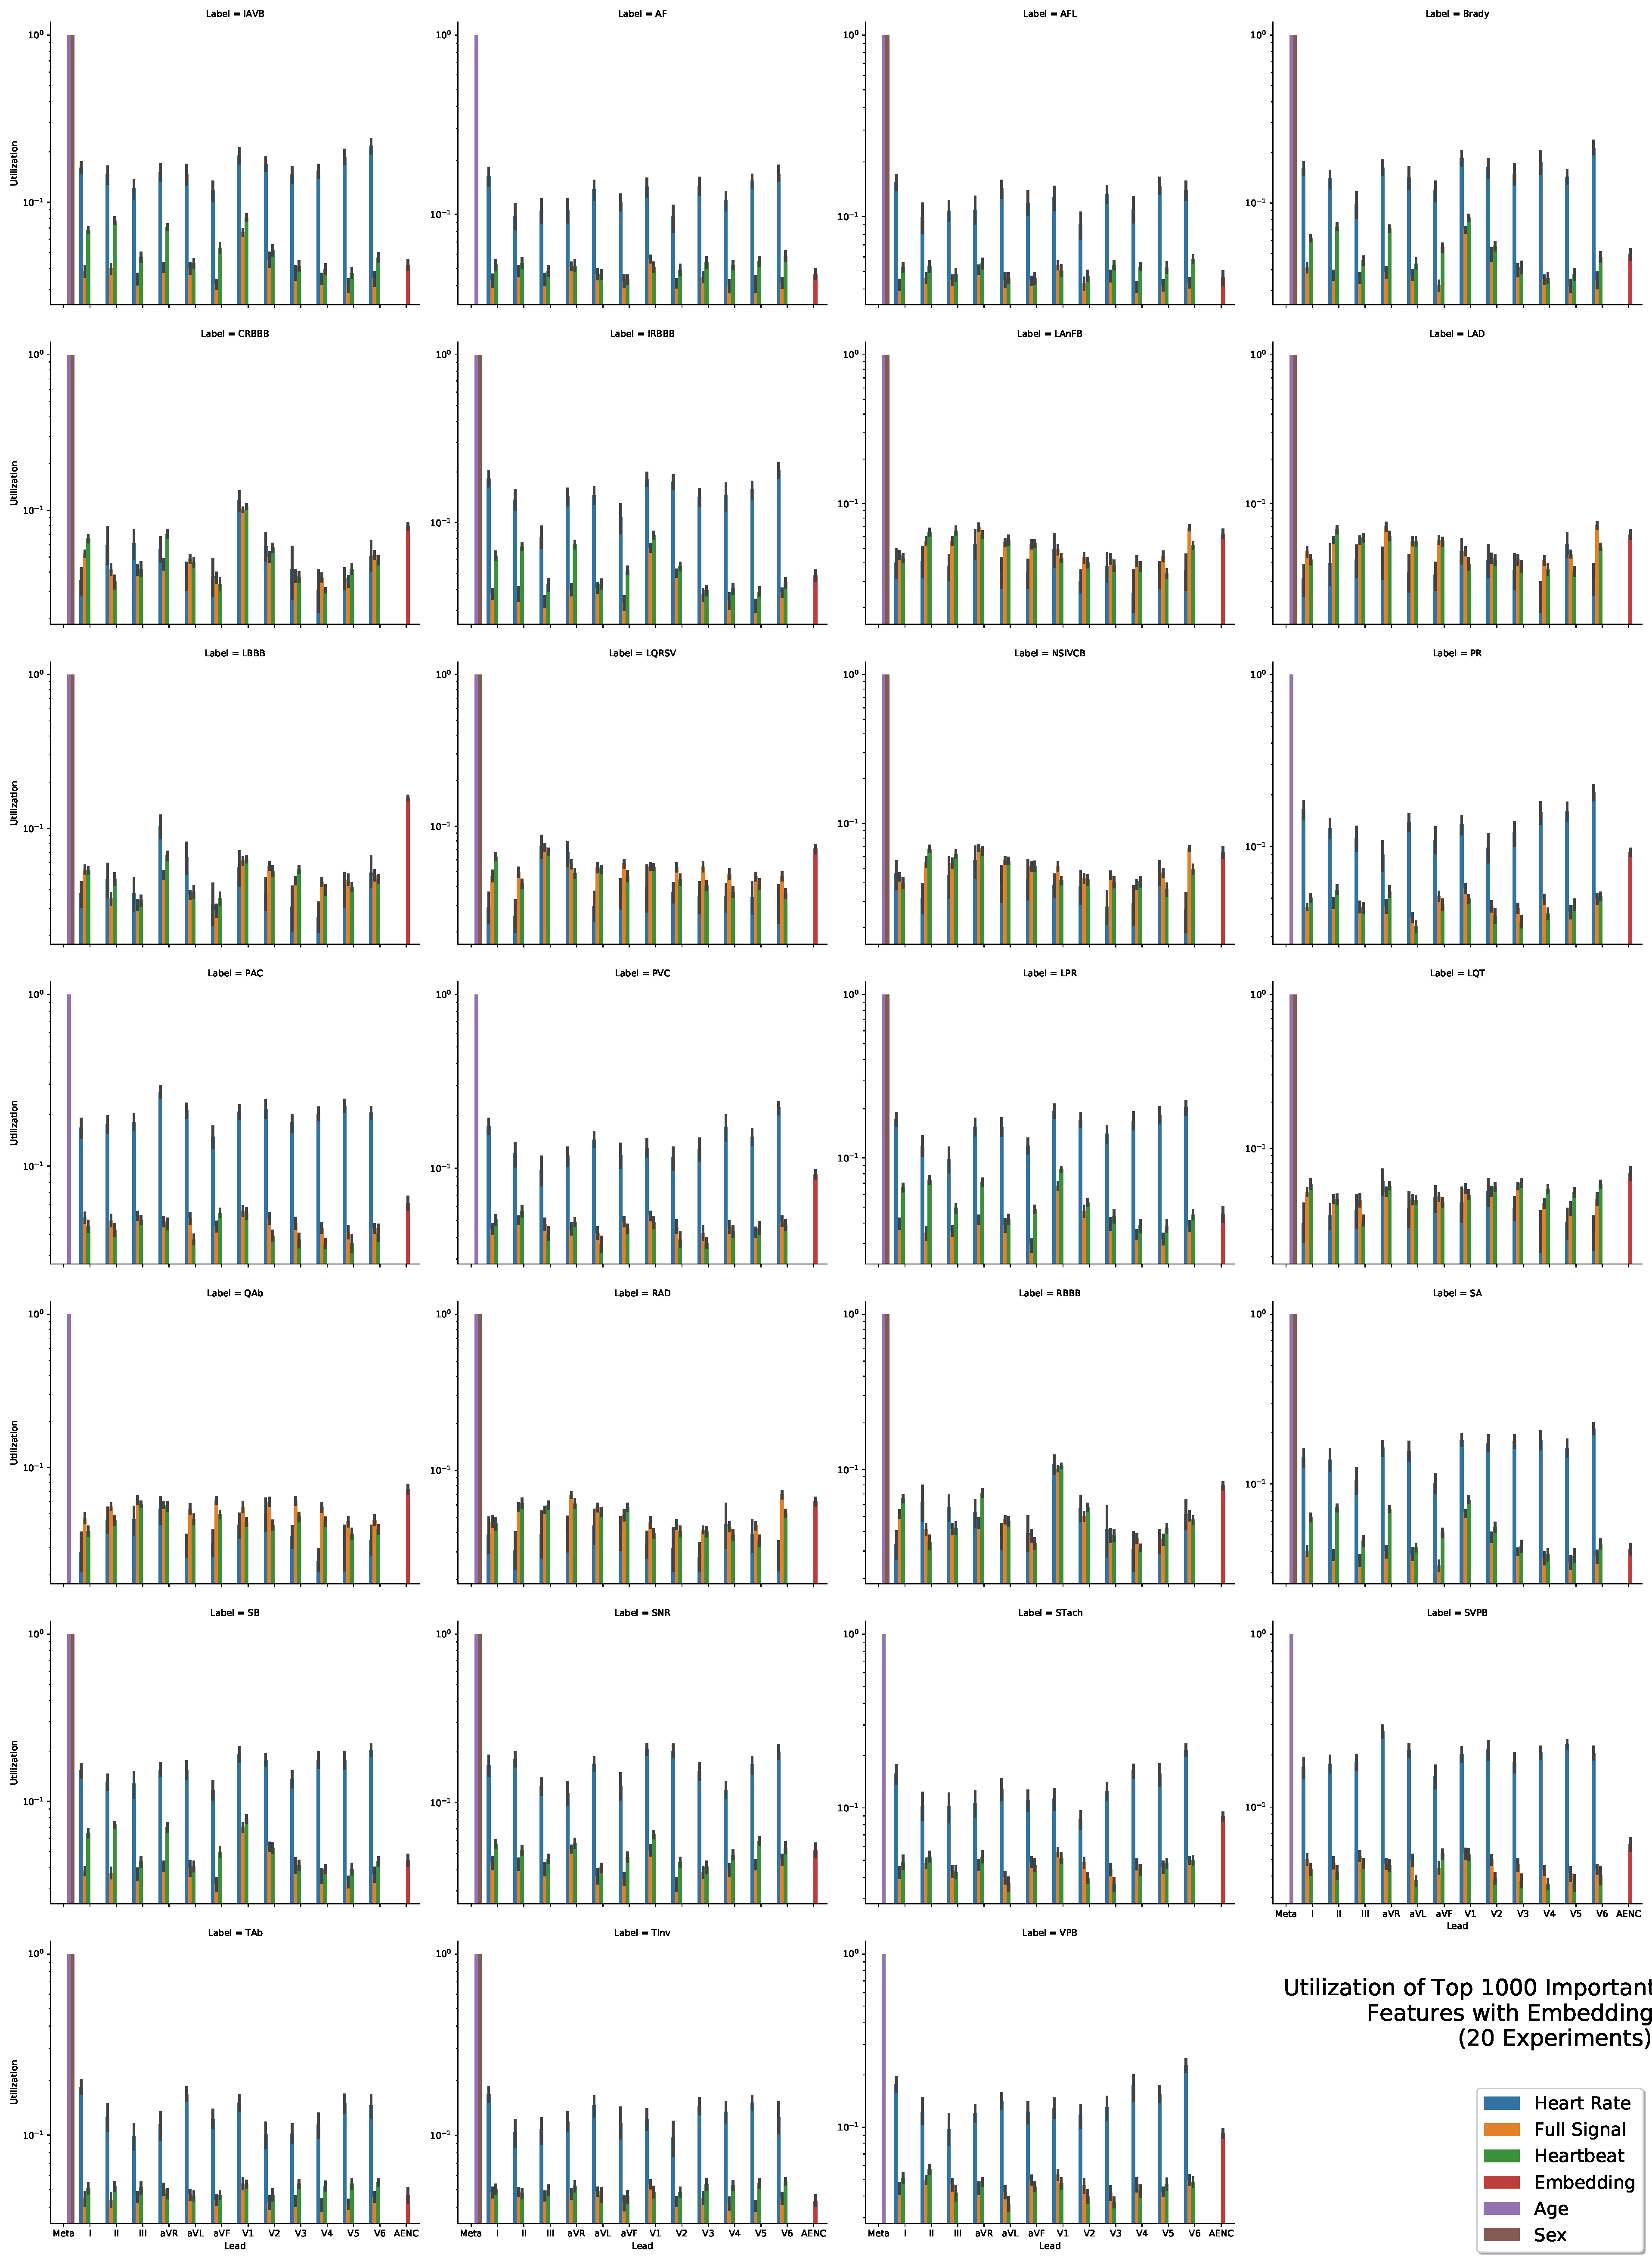
\includegraphics[width=\textwidth]{figure/utilization_top_1000_feature_importances_all_w_embedding.pdf}
    \caption{Feature importances summary of Configuration~\ref{item:xgb_aenc_model_top_1000_w_embd}: ``Top 1000 Features with Embeddings", aggregated utilization over 20 independent experiments. Each of the 27 diagnosed labels displayed separately, showcasing feature derived lead (alternatively Meta or Autoencoder), and category (heart rate, full waveform signal, heartbeat, embedding, age, sex).}
    \label{fig:xgb_aenc_top_1000_features_labelwise}
\end{figure}

Question~\ref{question:xgb_aenc_embd_ratio} asks whether or not the embeddings, when added to the classifier inputs, are actually used when classifying the cardiac diagnoses.
A categorical breakdown of the feature importances from Configuration~\ref{item:xgb_aenc_model_top_1000_w_embd}, showcasing label-wise counts of the feature derived lead and category types, can be found in Figure~\ref{fig:xgb_aenc_top_1000_features_labelwise}.
Counting the contribution of the autoencoder embedding features, we see that for the \gls{lbbb} and \gls{qab} diagnoses, the utilization of embedding features exceed the heartbeat, heart rate, and full waveform feature contributions of any other lead.
The top 100 important features variant from Configuration~\ref{item:xgb_aenc_model_top_100_w_embd} is displayed in Figure~\ref{fig:xgb_aenc_top_100_features_labelwise}.
In comparison, the utilization of autoencoder embedding features have diminished and no longer exceeds the other leads in any category in any label.

This suggests that the majority of the dominant important features are not provided by the autoencoder embeddings when feature pruning is aggressive (top 100).
When feature pruning is less aggressive (top 1000), the embedding features are more dominant than any other lead category in predicting \gls{lbbb} and \gls{qab}.

\begin{figure}[t]
    \centering
    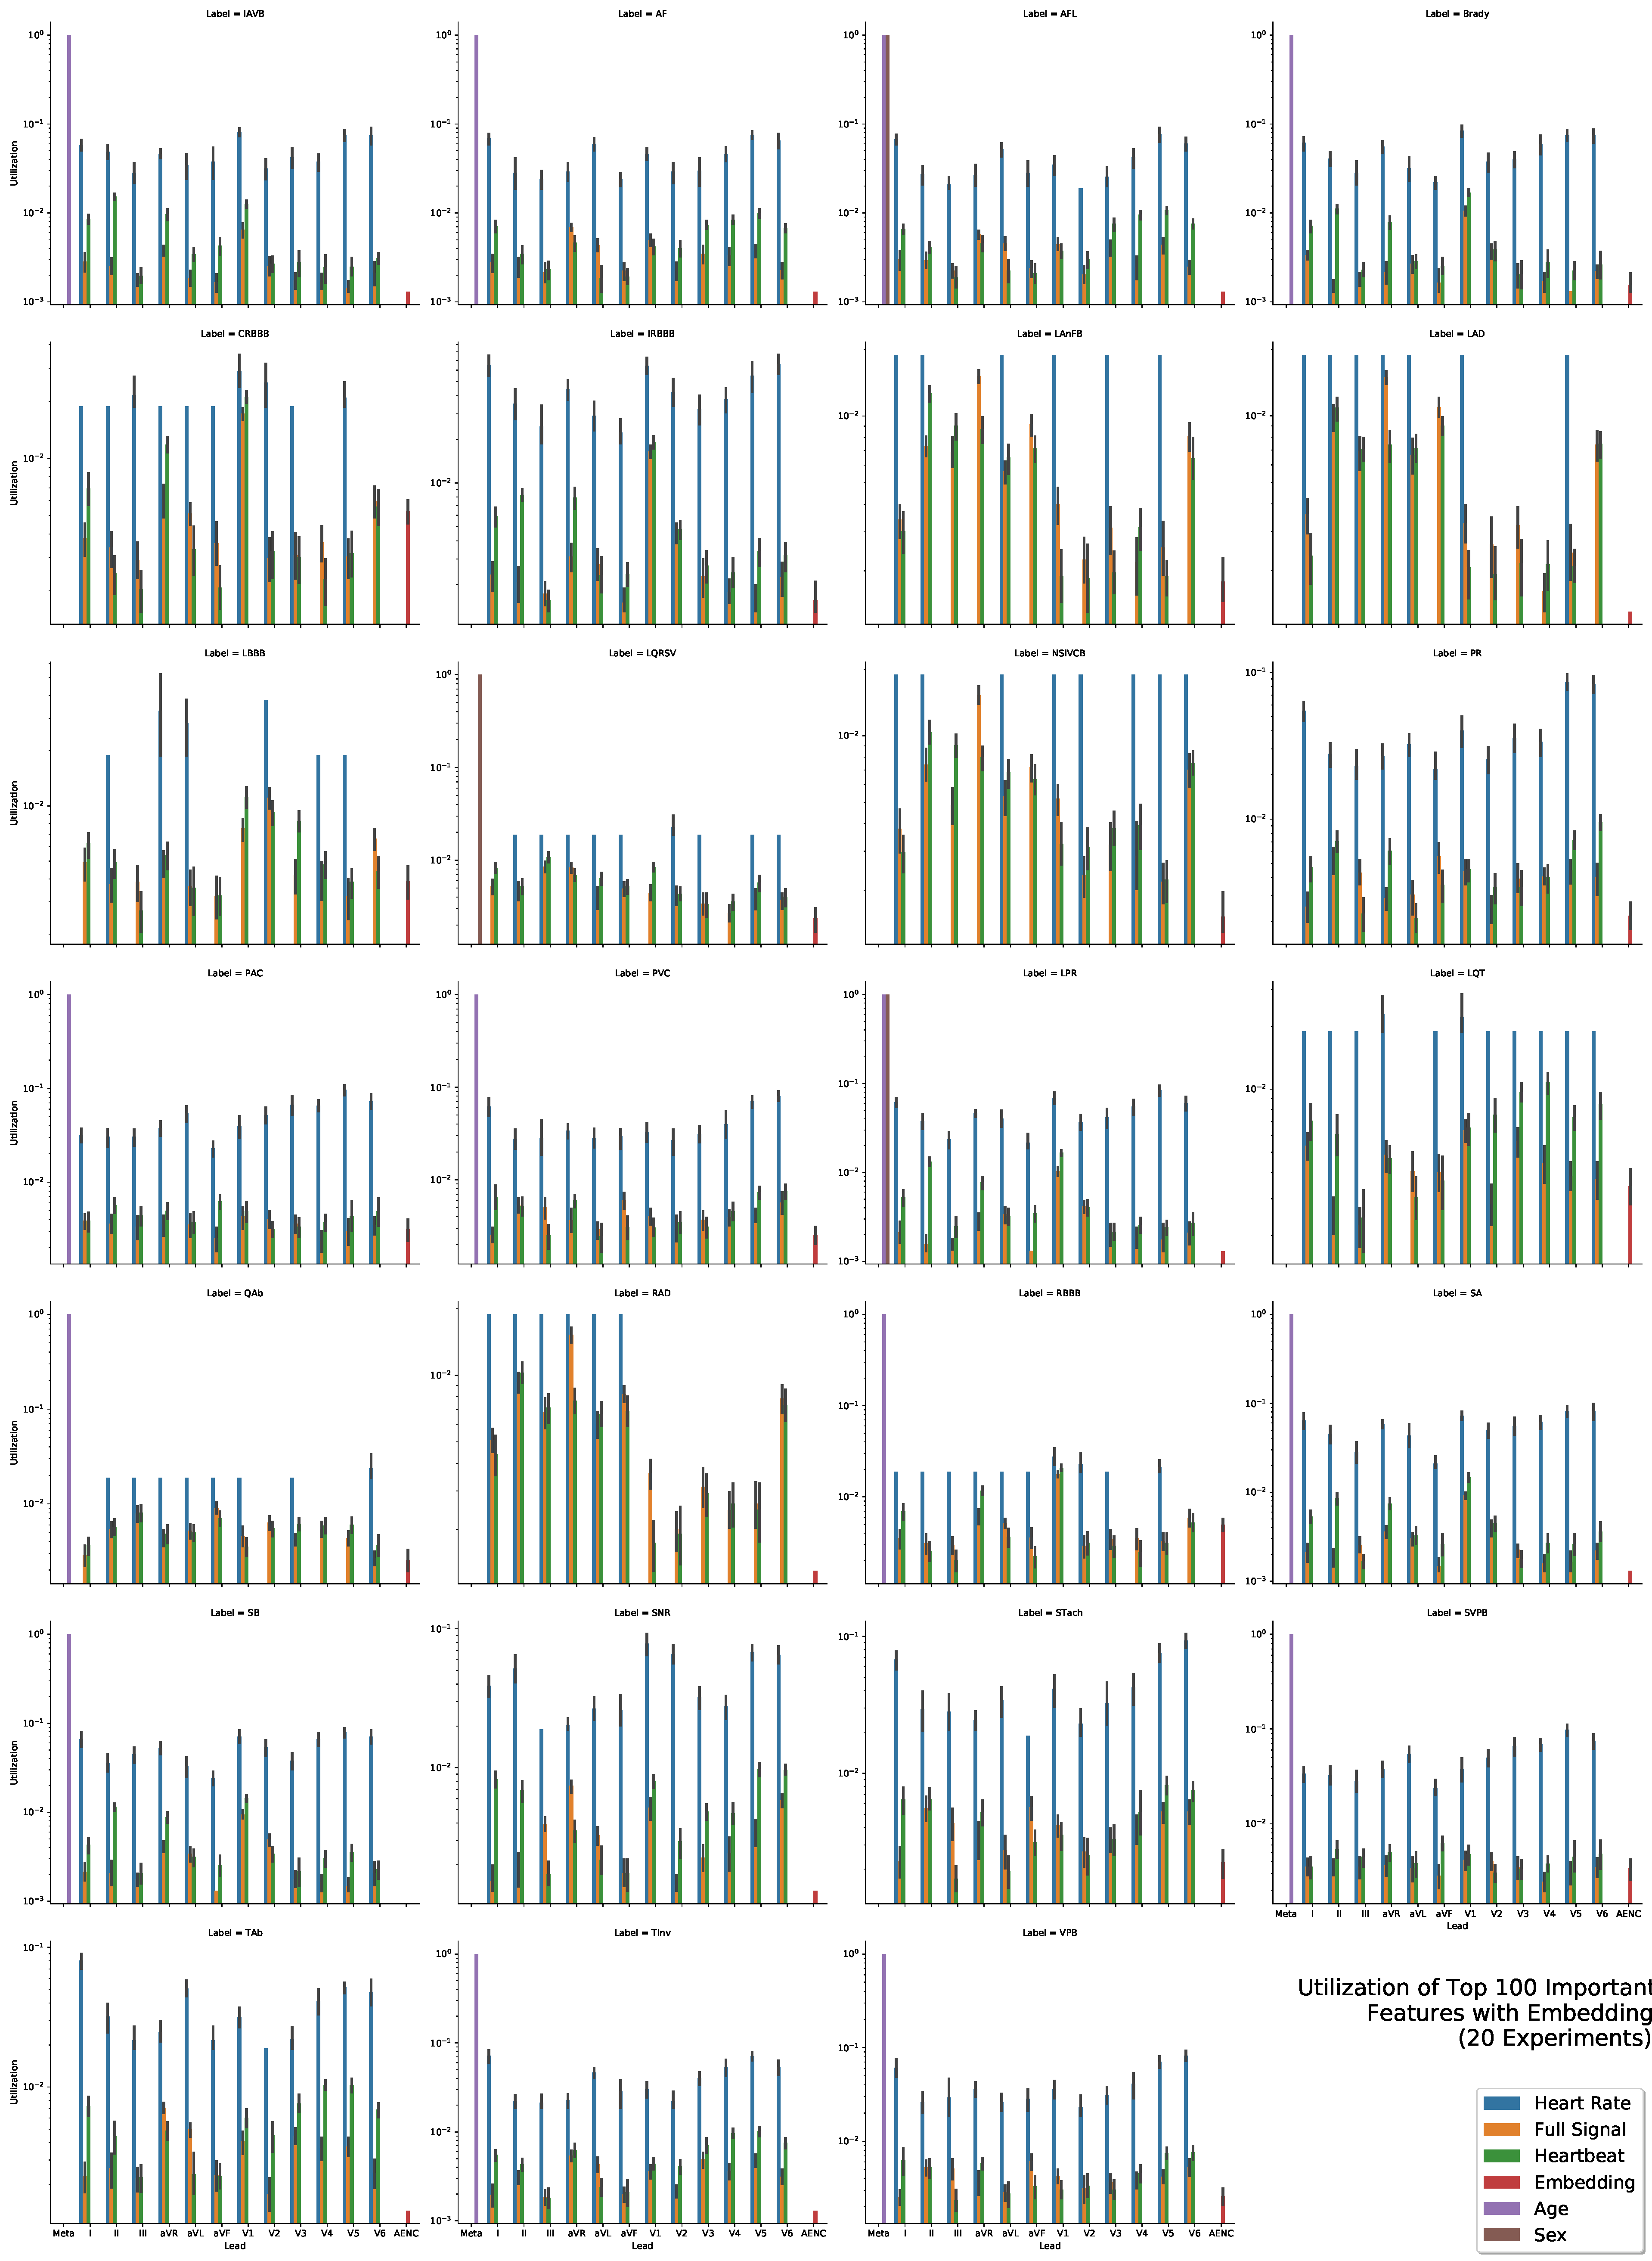
\includegraphics[width=\textwidth]{figure/utilization_top_100_feature_importances_all_w_embedding.pdf}
    \caption{Feature importances summary of Configuration~\ref{item:xgb_aenc_model_top_100_w_embd}: ``Top 100 Features with Embeddings", aggregated utilization over 20 independent experiments. Each of the 27 diagnosed labels displayed separately, showcasing feature derived lead (alternatively Meta or Autoencoder), and category (heart rate, full waveform signal, heartbeat, embedding, age, sex).}
    \label{fig:xgb_aenc_top_100_features_labelwise}
\end{figure}


\section{Discussion}

Bengio discusses in an informal academic research panel~\cite{2020-yoshua-dlc} current and upcoming deep learning challenges, where he dismisses the viability of engineering deep learning models into old-fashioned symbolic machine learning methods, instead proposing learned attention mechanisms as a viable alternative.
This is enforced by the experiment results, as no significant improvement in challenge metric can be attributed to the addition of autoenoder embedding representations alone.
Additionally, although the engineering of the two different mechanisms into one shallow machine learning classifier is feasible, we obscure the semantics of feature importance for the embedding features.
It is no longer clear how to trace the importances assigned to the embedding features back to their original lead sources.

The public dataset provided by the challenge contained notable irregularities that were not corrected when training the models.
Example irregularities include: 
\begin{itemize}
    \item \gls{ecg} records containing voltage over time changes exceeding physiologically possible voltage measurements
    \item \gls{ecg} records with miniscule voltage gain, peaks undiscernible from noise;
    \item \gls{ecg} records not labeled as \gls{brady} despite having resting heart rate of below 60 beats per minute;
    \item \gls{lqrsv} \gls{ecg} records incorrectly labeled as \gls{af}, \gls{tab}, or \gls{snr};
    \item \gls{tab} labeled \gls{ecg} records undiscernible from noise;
    \item inconsistent dataset labeling of \gls{af} and \gls{afl};
\end{itemize}
Additional improvements in the quality of the underlying dataset and the discarding of unusable \gls{ecg} records would likely improve the performance of the classifiers.

For future work, a replication of this study using other shallow classifiers, such as support vector machines, could provide insight into the relative effectiveness of the gradient boosted trees.
Using a wide set of tabular features per \gls{ecg} record appears to be inefficient, as feature pruning was the most useful regularization technique for improving the challenge metric score.
Expert domain specific knowledge for feature generation and selection may prove to be a more effective approach than distilling features from a general purpose time series feature extraction library.

Additionally, the challenge provided dataset contained an additional 88 unused classification labels.
Future work could consider applying these unused labels as additional features for classification in a gambit to learn diagnosis correlations or interactions.

\end{document}
